
\documentclass[12pt,letterpaper]{ntdhw}

\usepackage{graphicx}
\graphicspath{ {./images/} }



\title{Project 0: Functional Programming and Lisp Introduction}
\author{CSCI 561}

\rhead{Names: Luke Beukelman, Ben Breisch, Luc Lafave, Adam Thistlewood}

%\keytrue

\begin{document}
\pagestyle{fancyplain}

\maketitle
\thispagestyle{fancyplain}
%\clearpage

\begin{enumerate}

  \item What are the result types of the following Lisp expressions?
  \begin{enumerate}
    \item {\tt 1} : \emph{
      INTEGER
    }
    \item {\tt (+ 1 2)} : \emph{
      INTEGER
    }
    \item {\tt '(+ 1 2)} : \emph{
      LIST
    }
    \item {\tt (eval '(+ 1 2))} : \emph{
      INTEGER
    }
    \item {\tt (lambda () (+ 1 2))} : \emph{
      FUNCTION
    }
    \item {\tt "foo"} : \emph{
      STRING/ARRAY
    }
    \item {\tt 'bar} : \emph{
      SYMBOL
    }
  \end{enumerate}

  \item Tail Calls:
  \begin{enumerate}
    \item What is tail recursion?

    \begin{emph}
      Answer: Tail recursion occurs when the recursive call is the last operation of a function.
      In tail recursion, rather than creating a new stack frame, the compiler may optimize the code
      so that the current stack frame is replaced, resulting in fewer memory allocations and faster
      performance.
    \end{emph}

    \item In the recursive implementation, will {\tt fold-left} or
    {\tt fold-right} be more memory-efficient?  Why?

    \begin{emph}
      Answer: Fold-left will be more memory efficient because it is tail recursive, and fold-right uses a large function call stack while fold-left processes on the go.
    \end{emph}
  \end{enumerate}

  \item Lisp and Python represent code differently.

  \begin{enumerate}
    \item Contrast the representations of Lisp code and Python code.

    \begin{emph}
      Answer: Lisp and Python are different in many aspects. Lisp code uses S-expressions for the syntax of its code. This uses many parentheses in its design. This may be hard to read if unfamiliar with the language.         Python on the other hand is written to be familiar to most programmers by using indentation instead of Lisp's parentheses. This is a more common type of syntax. Many believe that Python has the shortest syntax but 
      Lisp actually is less at times. For example, in Lisp there is no need for the phrases 'return' or 'else'. Although Lisp can be used for multiple types of programming, it is more well known for being a functional 
      programming language. This allows it to process proofs and theory better. It is also more well known for its ability to do symbolic computing. Python is known for being multifaceted. From data analysis, to 
      scripting, to object-oriented programming, to even web development, Python has the ability to cover more areas of programming more effectively then Lisp. Python is the more popular language today so it provides 
      more libraries and frameworks then Lisp. To summarize this paragraph, Lisp and Python have different syntax, excel in different areas, and vary in popularity today. 
    \end{emph}

    \item How do Python's {\tt eval()} and {\tt exec()} differ from
    the approach of Lisp?

    \begin{emph}
      Answer: Python's {\tt eval()} and {\tt exec()} functions are used to run code dynamically like Lisp. This means that they can type-change during run-time. This is a very powerful tool to be able to do. Python's is 
      different than Lisp for a few reasons. Both of Python's methods require a string as an input. That is what the code is stored in. In Lisp the code needs to be written in an S-expression but the type does not 
      matter. When the code chunk is ran in Python, with these methods, the output is not outputted automatically. Where in Lisp, the output is shown after execution. 
    \end{emph}
  \end{enumerate}

  \item GCC supports an extension to the C language that allows
  local/nested functions (functions contained in other functions).  A
  GCC local function can access local variables from its parent
  function.
  \begin{enumerate}
    \item What problems could arise if you return a function pointer
    to a GCC local function? \emph{(Hint: ``Funarg problem'')}

    \begin{emph}
      Answer: % Your Answer Here
      GCC languages are compiled and don't have managed environments, so a function passed by pointer
      would not be able to access local variables, as it would be compiled irrelevant of the
      scope/environment in which the local variables are declared. 

    \end{emph}

    \item How does Lisp handle this problem?

    \begin{emph}
      Answer: Lisp, having a runtime and treating functions as first-class objects, can create
      a complexity of the lexical environment and provide it for the function to run.
    \end{emph}

  \end{enumerate}


  \item Test the performance of your implementation of
    \texttt{merge-sort}.
    \begin{enumerate}
    \item Plot the running time of your \texttt{merge-sort}
      implementation for increasing input sizes.  Include enough data
      points to demonstrate the empirical asymptotic running time.

    \begin{emph}
      Answer: % Your Answer Here 
      \break 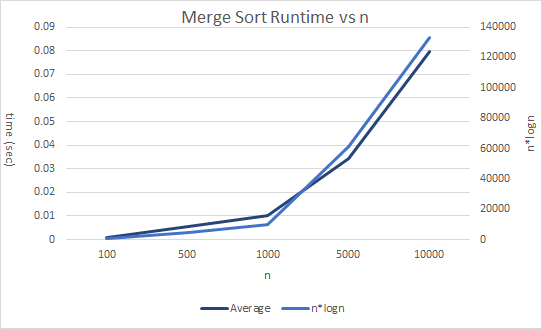
\includegraphics{merge} \break
      The graph above shows the average of 5 runs of merge-sort for an increasing value of n,
      on a processor clocked at 2.2 Ghz. Values within a test list of length n were generated using
      Common Lisp's \(RANDOM\) function. The graph also shows a theoretical \(n*log(n)\) on a secondary axis.
      
    \end{emph}

    \item What asymptotic running time did you expect for
      \texttt{merge-sort}, and what running time did you observe?
      Explain any differences.

    \begin{emph}
      Answer: % Your Answer Here
      Merge-sort has an average runtime complexity of \(\theta (n*log(n))\). As you can see in the graph above, the runtime of our algorithm very nearly matches the theoretical complexity of the algorithm. Some explanations for the small amount of error include CPU clock speed variations, scheduling discrepancies, as well as competing processes. All development and testing was done on Isengard, a shared server that has many users.
    \end{emph}

    \end{enumerate}

\end{enumerate}

\end{document}

%%% Local Variables:
%%% mode: latex
%%% TeX-master: t
%%% End:
